\documentclass[aspectratio=169]{beamer}

\usepackage[utf8]{inputenc}
\usepackage{default}

\setbeamertemplate{navigation symbols}{}


\usetheme{Montpellier}

%\beamersetuncovermixins{\opaqueness<1>{25}}{\opaqueness<2->{15}}

\title{ Geladenes Teilchen im elektrischen Feld }  
\author{ Michael Cerny \& Stefan Schindler }
\date{ 4. M\"arz 2015 } 

\begin{document}
\begin{frame}
  \titlepage
\end{frame}

\begin{frame}
  \frametitle{ Inhalt }
  \tableofcontents
\end{frame}

\section{ Grundkonzept St\"orungstheorie } 
\begin{frame}\frametitle{ Grundkonzept St\"orungstheorie } 
  \section{ Potentialkasten mit eFeld }
  \[
  \hat{H} = \varepsilon^0 \hat H_0 + \varepsilon^1 \hat H_1 + \ldots + \varepsilon^\infty \hat H_\infty
  \]
\end{frame}

\section{ Modell der St\"orung }
\begin{frame}
  \frametitle{ Modell der St\"orung }
  \begin{figure}
    \centering
    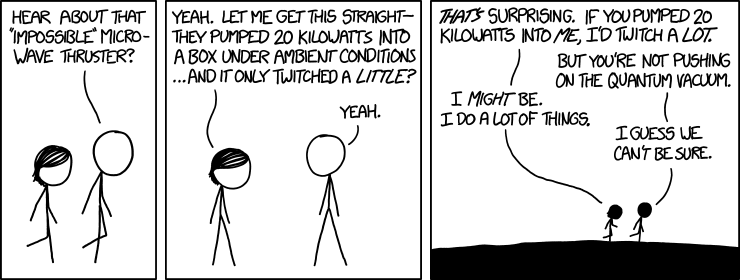
\includegraphics[width=14cm]{./1404_quantum_vacuum_virtual_plasma.png}
    % 1404_quantum_vacuum_virtual_plasma.png: 0x0 pixel, 0dpi, 0.00x0.00 cm, bb=
    \caption{xkcd 1404 \textendash \ Quantum Vacuum Virtual Plasma}
    \label{abb:1404_quantum_vacuum_virtual_plasma}
  \end{figure}

\end{frame}


\subsection{ Ungest\"orter Teil }
\begin{frame}
  \frametitle{ Ungest\"orter Teil }
  Als $\hat H_0$ nehmen wir
  \[
    \hat H_0 = \frac{\hbar^2}{2m} \frac{\partial^2}{\partial x^2} + V_0(x)
  \]
  f\"ur das Potential $V_0(x)$ gilt
  \[
    V_0(x)=\begin{cases}
      0       & \qquad |x|<l\\
      \infty  & \qquad\text{sonst.}
    \end{cases}
  \]
\end{frame}

\subsection{ 1. N\"aherung der St\"orung }
\begin{frame} 
  \frametitle{ 1. N\"aherung der St\"orung }

  F\"ur $\hat H_1$ gilt
  \[
    \hat H_1 = \frac{\hbar^2}{2m} \frac{\partial^2}{\partial x^2} + V_1(x)
  \]

  f\"ur das Potential $V_1(x)$ gilt
  \[
    V_1(x) = a*x +b ; b = 0 \text{ weil es dann symetisch ist }
  \]

  Die Ausgangsgleichung f\"ur $\hat{H}$ lautet
  \[
    \hat{H} = \varepsilon^0 ( \frac{\hbar^2}{2m} \frac{\partial^2}{\partial x^2} + V_0(x) )
	      + \varepsilon^1 ( \frac{\hbar^2}{2m} \frac{\partial^2}{\partial x^2} + a*x )
  \]
\end{frame}


\section{ Gleichungen Umformen }
\begin{frame}
  \frametitle{ Gleichungen Umformen }
  \begin{figure}
    \centering
    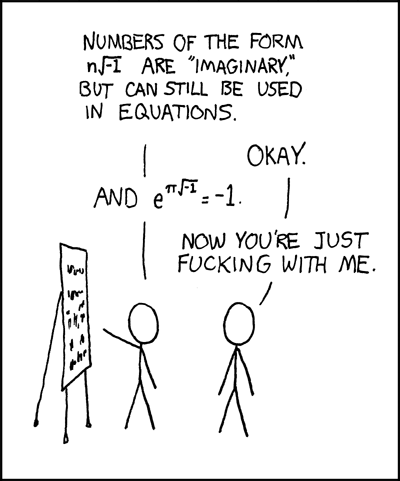
\includegraphics[height=5.6cm]{./179_e_to_the_pi_times_i.png}
    % 179_e_to_the_pi_times_i.png: 0x0 pixel, 0dpi, 0.00x0.00 cm, bb=
    \caption{ xkcd 1404 \textendash \ e to the pi times i }
    \label{abb:179_e_to_the_pi_times_i}
  \end{figure}
\end{frame}

\section{ Bilder }
\subsection{ Psi ungest\"ort }
\begin{frame}
  \frametitle{ Bilder }
  \begin{figure}
    \centering
    % [clip=true,trim=links unten rechts oben]
    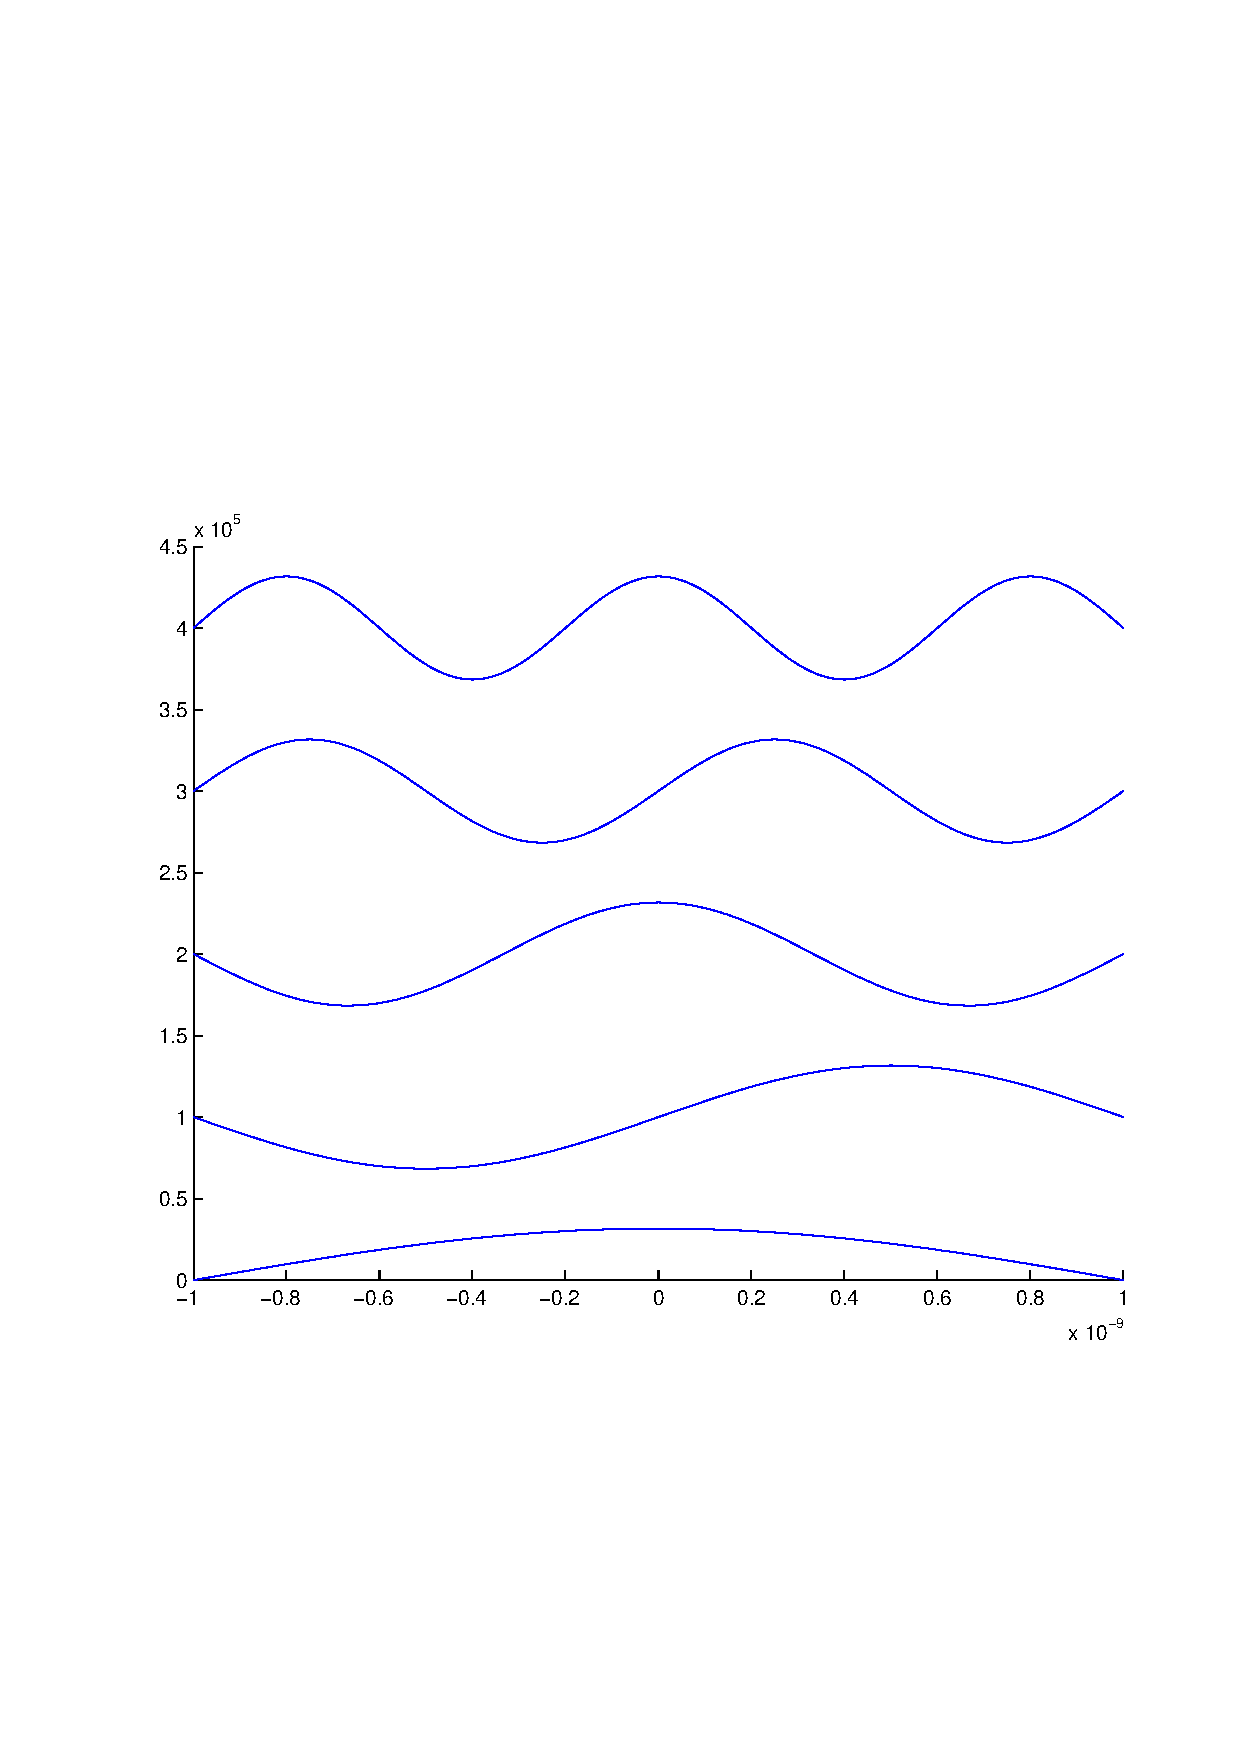
\includegraphics[height=5.6cm,clip=true,trim=2cm 7.5cm 1cm 8cm]{../../skript/efeld/Psi_ungestoert.pdf}
    \caption{$\psi$ ungest\"ort}
    \label{abb:efeld_psi_ungestoert}
  \end{figure}

\end{frame}

\subsection{ Psi gest\"ort }
\begin{frame}
  \frametitle{ Bilder }
  \begin{figure}
    \centering
    % [clip=true,trim=links unten rechts oben]
    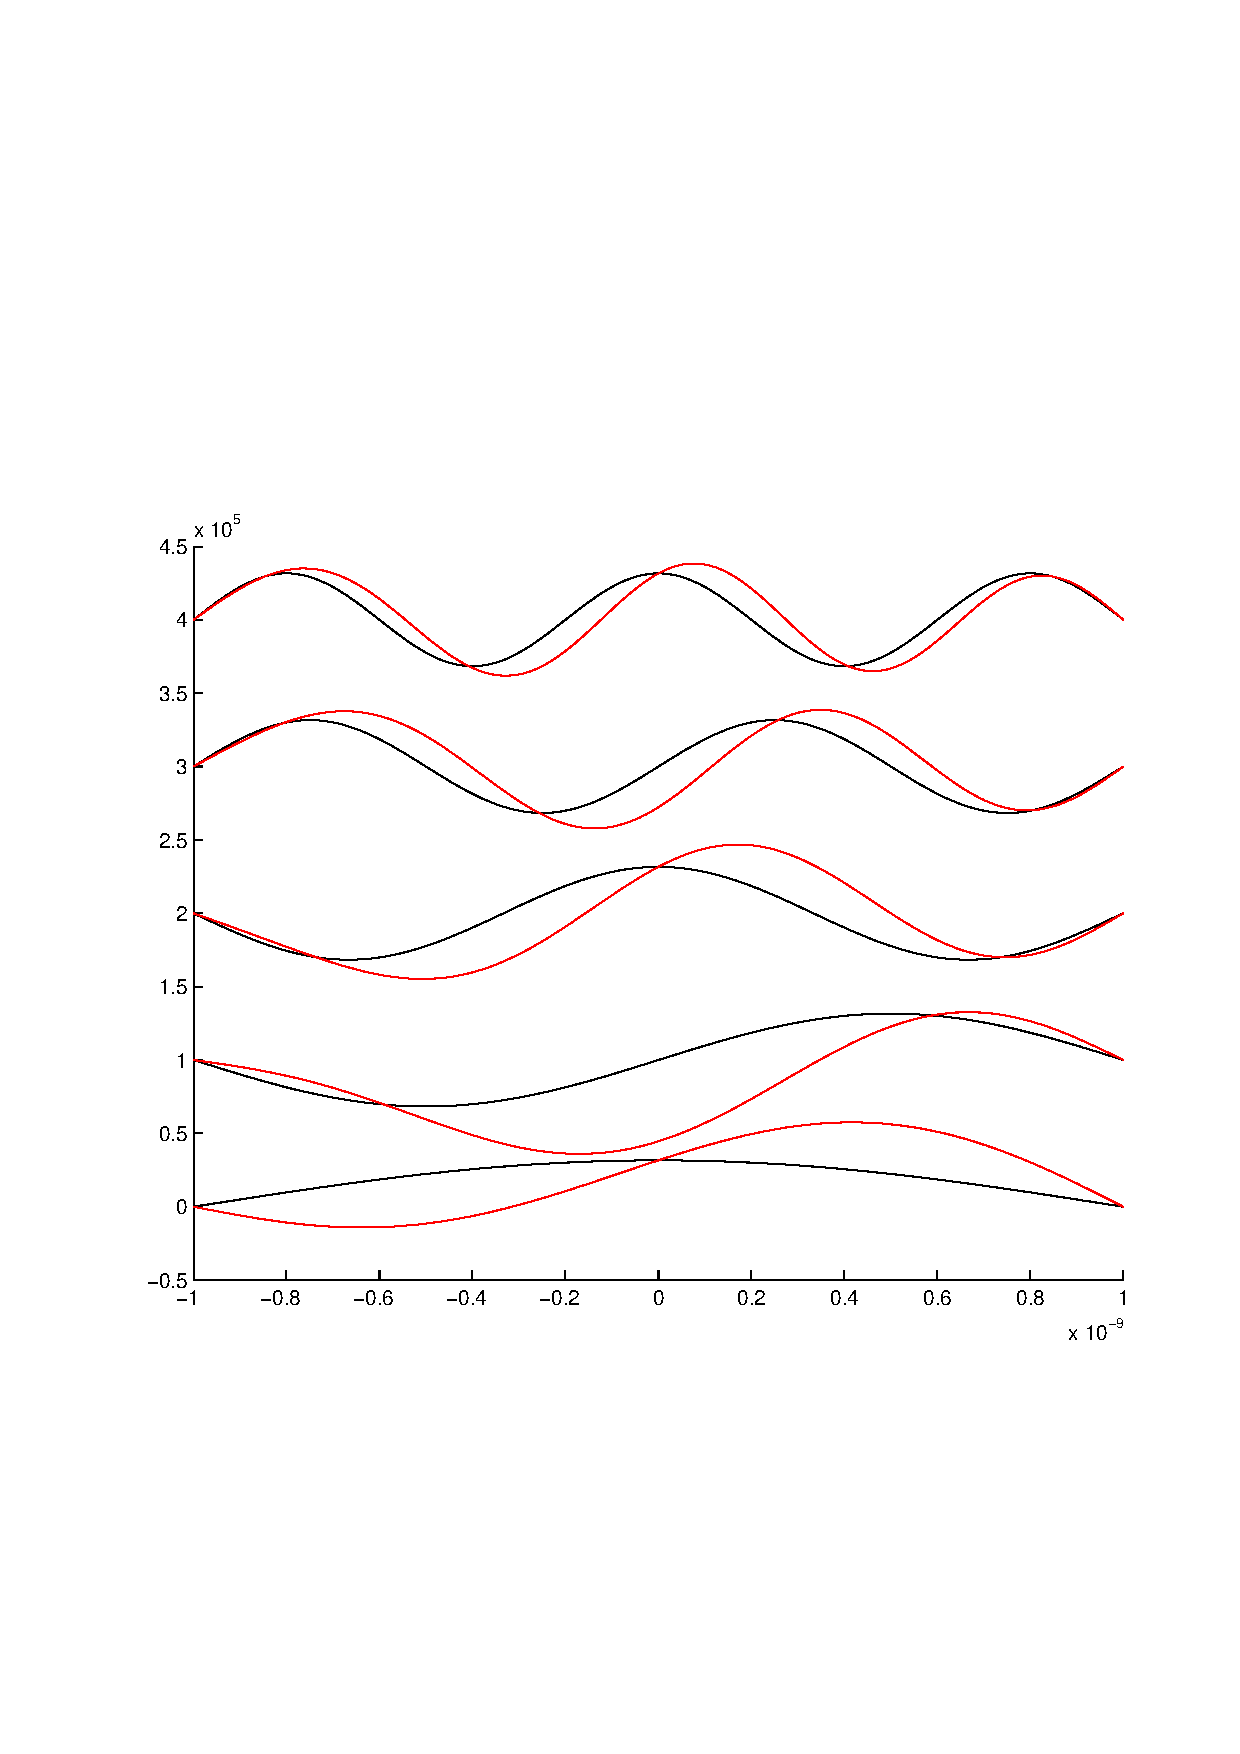
\includegraphics[height=5.6cm,clip=true,trim=2cm 7.5cm 1cm 8cm]{../../skript/efeld/Psi_gestoert.pdf}
    \caption{$\psi$ gest\"ort}
    \label{abb:efeld_psi_gestoert}
  \end{figure}

\end{frame}




\section{ Fragen }
\begin{frame}
  \frametitle{ Fragen }
\end{frame}


\end{document}
